\chapter{Từ trường của dòng điện chạy trong dây dẫn uốn thành vòng tròn}
\section{Lý thuyết trọng tâm}
\subsection{Đường sức từ tạo bởi dòng điện qua dây dẫn uốn thành vòng tròn}
Là những đường có trục đối xứng là đường thẳng qua tâm vòng dây và vuông góc với mặt phẳng chứa vòng dây.
\begin{center}
	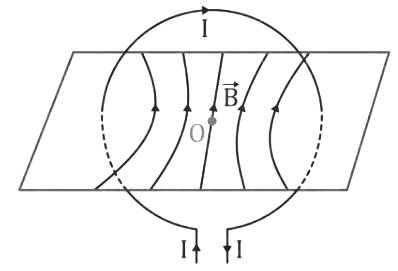
\includegraphics[scale=1]{../figs/VN11-PH-26-L-018-2-h88.jpg}
\end{center}
\subsection{Véctơ cảm ứng từ $\vec{B}$ do dòng điện chạy trong khung dây tròn gây ra tại tâm của vòng dây}
\begin{itemize}
	\item Điểm đặt: tại tâm vòng dây.
	\item Phương: vuông góc với mặt phẳng chứa vòng dây. 
	\item Chiều: xác định theo quy tắc nắm tay phải hoặc vào Nam ra Bắc.
	
	Nắm tay phải theo chiều dòng điện trong khung, khi đó ngón cái chỉ hướng của các đường sức từ đi qua phần mặt phẳng giới bởi vòng dây.
	
	\item Độ lớn:  
	\begin{equation}
	B=2\pi\cdot 10^{-7}\cdot N\cdot \dfrac{I}{R},
	\end{equation}
	trong đó,
	\begin{itemize}
		\item $N$ là số vòng dây.
		\item $I$ là cường độ của dòng điện, đơn vị ampère (A). 
		\item $R$ là bán kính của khung dây tròn, đơn vị mét (m). 
		\item $B$ là cảm ứng từ, đơn vị tesla (T).
	\end{itemize}
	
\end{itemize}

\subsection{Nguyên lý chồng chất từ trường}
Véctơ cảm ứng từ tại một điểm do nhiều dòng điện gây ra bằng tổng các véctơ cảm ứng từ do từng dòng điện gây ra tại điểm đó
\begin{equation}
\vec{B}=\vec{B}_1+\vec{B}_2+\vec{B}_3+...+\vec{B}_\text{n},
\end{equation} 
trong đó, $\vec{B}_1, \ \vec{B}_2, \ \vec{B}_3,..., \ \vec{B}_\text{n}$ là cảm ứng từ do các dòng điện $I_1, \ I_2, \ I_3,..., \ I_\text{n}$ gây ra tại điểm đang xét.

\section{Bài tập}
\begin{dang}{Công thức cảm ứng từ $\vec{B}$ do dòng điện qua khung dây tròn gây ra tại tâm của vòng dây}
\end{dang}

\textbf{Phương pháp giải}

Áp dụng công thức  $B=2\pi \cdot 10^{-7}\cdot N \cdot \dfrac{I}{R}$, từ đó tìm được giá trị cảm ứng từ $B$, số vòng dây $N$, cường độ dòng điện $I$,  bán kính $R$ khung dây tròn.

\vspace{1em}
{
	\vidu{2}{
	
	Khung dây tròn có 20 vòng, bán kính là $\text{3,14}\ \text{cm}$. Khi có dòng điện đi vào thì tại tâm của vòng dây xuất hiện từ trường là $B=2\cdot 10^{-3}\ \text{T}$. Tính cường độ dòng điện trong vòng dây.
	\begin{mcq}(4)
		\item $\text{3}\ \text{A}$.
		\item $\text{4}\ \text{A}$.
		\item $\text{5}\ \text{A}$.
		\item $\text{6}\ \text{A}$.
	\end{mcq}
	}{
\begin{center}
		\textbf{Hướng dẫn giải:}
\end{center}

	$B=2\pi \cdot 10^{-7}\cdot N \cdot \dfrac{I}{R}$
	
	$\Rightarrow I=B\cdot \dfrac{R}{2\pi \cdot 10^{-7}\cdot N }=\text{5}\ \text{A}$.
	
	Vậy cường độ dòng điện trong vòng dây là 5 A.
	
\textbf{	Đáp án: C.}}
}

{\viduii{3}{
	
Hai sợi dây đồng giống nhau được uốn thành hai khung dây tròn, khung thứ nhất chỉ có một vòng, khung thứ hai có 2 vòng. Nối hai đầu mỗi khung vào hai cực của mỗi nguồn điện để dòng điện chạy trong mỗi vòng của hai khung là như nhau. Hỏi cảm ứng từ tại tâm của khung nào lớn hơn và lớn hơn bao nhiêu lần?
	\begin{mcq}(4)
		\item $B_2=2B_1$.
		\item $B_1=2B_2$.
		\item $B_1=4B_2$.
		\item $B_2=4B_1$.
	\end{mcq}}
{	
\begin{center}
		\textbf{Hướng dẫn giải:}
\end{center}
	
	Hai sợi dây giống nhau nên sẽ có cùng chiều dài $l$.
	
	$\Rightarrow l=2\pi\cdot R_1=2\cdot \left( 2\pi \cdot R_2\right)\Rightarrow R_1=2R_2$.
	
	$B_1=2\pi\cdot N_1 \cdot 10^{-7}\dfrac{I}{R_1}$, 	$B_2=2\pi\cdot N_2 \cdot 10^{-7}\dfrac{I}{R_2}$.
	
	$\Rightarrow \dfrac{B_2}{B_1}=\dfrac{R_1}{R_2}\cdot \dfrac{N_2}{R_1}=4$.
	
	
	$\Rightarrow B_2=4B_1$.
	
\textbf{	Đáp án: D}
}}


\begin{dang}{Tổng hợp véctơ cảm ứng từ $\vec{B}$ bởi dòng điện thẳng dài và khung dây tròn}
\end{dang}

\textbf{Phương pháp giải}
\begin{description}
	\item[Bước 1:] Xác định điểm đặt, phương, chiều của véctơ cảm ứng từ $\vec{B}$ do các dòng điện thẳng và khung dây tròn gây ra tại điểm đang xét bằng quy tắc nắm tay phải.	
	\item[Bước 2:] Sử dụng công thức tính cảm ứng từ bởi dòng điện thẳng dài $B=2\cdot 10^{-7}\dfrac{I}{r}$ và cảm ứng từ bởi dòng điện chạy qua khung dây tròn $B=2\pi\cdot N \cdot 10^{-7}\dfrac{I}{R}$. 
	\item[Bước 3:] Áp dụng quy tắc tổng hợp véctơ và nguyên lý chồng chất từ trường để xác định véctơ cảm ứng từ $\vec{B}$ tổng hợp tạo bởi nhiều dòng điện.
\end{description}
\vspace{1em}
{\vidu{3}{	
	Một dây dẫn thẳng, dài có vỏ bọc cách điện, ở khoảng giữa được uốn thành vòng tròn, bán kính $R=   20\ \text{cm}$ như hình vẽ. Dòng điện chạy qua dây dẫn có cường độ 5 A. Xác định cảm ứng từ tại tâm O của vòng tròn.
	\begin{center}
		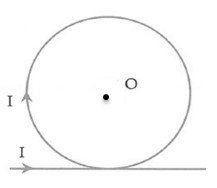
\includegraphics[scale=0.8]{../figs/VN11-PH-26-L-018-2-h89.jpg}
	\end{center}

	\begin{mcq}(4)
		\item $\text{5}\cdot 10^{-6}\ \text{T}$.
		\item $\text{10,7}\cdot 10^{-6}\ \text{T}$.
		\item $\text{15,7}\cdot 10^{-6}\ \text{T}$.
		\item $\text{20,7}\cdot 10^{-6}\ \text{T}$.
	\end{mcq}}{
\begin{center}
		\textbf{Hướng dẫn giải:}
\end{center}
	\begin{center}
		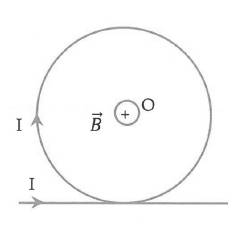
\includegraphics[scale=0.8]{../figs/VN11-PH-26-L-018-2-h90.jpg}
	\end{center}


Dòng điện chạy trong vòng tròn gây ra tại tâm O cảm ứng từ $\vec{B}_1$ vuông góc với mặt phẳng hình vẽ, hướng từ ngoài vào và có độ lớn:

\begin{equation}
B_1=2\pi\cdot N \cdot 10^{-7}\dfrac{I}{R}=\text{15,7}\cdot 10^{-6}\ \text{T}.
\end{equation}


Dòng điện chạy trong dây dẫn thẳng gây ra tại tâm O cảm ứng từ  vuông góc với mặt phẳng hình vẽ, hướng từ trong ra và có độ lớn: 

\begin{equation}
B_2=2\cdot 10^{-7}\dfrac{I}{R}=\text{5}\cdot 10^{-6}\ \text{T}.
\end{equation}

Cảm ứng từ tổng hợp tại O là $\vec{B}=\vec{B}_1+\vec{B}_2$.

Vì $\vec{B}_1$ và $\vec{B}_2$ cùng phương, ngược chiều và về độ lớn $B_1>B_2$.

Nên cảm ứng từ tổng hợp $\vec{B}$ cùng phương, cùng chiều với $\vec{B}_1$ và có độ lớn là:

\begin{equation}
 B=\left|B_1-B_2\right| =\text{10,7}\cdot 10^{-6}\ \text{T}.    
\end{equation}

\textbf{Đáp án: B}
}
	

